

% Capítulo 4
\chapter{Equações, Provas e Especificações}\label{cap:equa}

O intuito deste capítulo é o de introduzir os pacotes matemáticos que foram sugeridos por diversos professores, de acordo com suas necessidades, e mostrar exemplos simples de como usá-los. Ele não deve ser visto como texto introdutório, mediano ou avançado sobre como se deve usar os ambientes matemáticos disponíveis em \LaTeX{}. Existem vários excelentes livros e manuais físicos e digitais, pagos e gratuitos, que lidam com este extenso tópico, de modo que não usarei espaço neste capítulo para tal.

Como sugestões de referências sobre o uso de comandos e pacotes \LaTeX{} para a escrita de fórmulas matemáticas, elenco as seguintes:
\begin{enumerate}
	\item Short Math Guide for \LaTeX{} - Disponível em  \url{http://mirrors.ctan.org/info/short-math-guide/short-math-guide.pdf}
	\item \LaTeX{} Cookbook \parencite{Kottwitz2015} - Livro disponível em papel e eletronicamente.
	\item Overleaf - O \gls{overleaf}\index{Overleaf} separa pequenos textos introdutórios e com exemplos para diferentes tópicos relacionados à definição de equações. Um bom lugar para iniciar a leitura é \url{https://www.overleaf.com/learn/latex/mathematical_expressions}.
\end{enumerate}

\section{Equações}

Um dos principais objetivos de Knuth quando projetou o \TeX{} era o de permitir a construção de fórmulas matemáticas de modo simples, mas que tivessem qualidade profissional quando impressas. Então, ele definiu sintaxes para vários símbolos matemáticos e criou comandos para a representação de equações. 
Para que \TeX{} ou \LaTeX{} gere os símbolos matemáticos, eles precisam saber que o texto é matemático. Os textos matemáticos pode ser do tipo texto (ou \textit{inline}), isto é, os símbolos são colocados na linha de texto, ou equação, onde os símbolos são colocados na linha própria deles.

No caso dos textos matemáticos \textit{inline}, nós sinalizamos um texto matemático usando os delimitares \textbackslash ( e \textbackslash ), no caso do \LaTeX e \$ e \$, no caso do \TeX{} e \LaTeX{}. Deve-se ter cuidado para não colocar equações ou símbolos muito altos que acabem gerando em espaçamento muito grande entre linhas, o que pode gerar uma diagramação não agradável visualmente. Um exemplo de equação simples que pode caber em uma linha é \( E = m c^2 \), que foi gerada com o código
\texttt{\textbackslash ( E = mc\^{}2 \textbackslash )}.

Os textos matemáticos no formato equação podem ser numerados ou não. No caso das equações não numeradas, você pode usar os delimitadores \textbackslash [ e \textbackslash ] no caso do \LaTeX{} e \$\$ e \$\$, no caso do \TeX{} e \LaTeX{}. Caso esteja usando \texttt{amsmath}\index{amsmath} \parencite{amsmath} ou \texttt{mathtools}\index{mathtools} \parencite{mathtools}, você pode usar a versão ``*'' do ambiente \texttt{equation}, que suprime a numeração e contagem dos objetos. O mesmo vale para os outros ambientes definidos em \texttt{mathtools}, como \texttt{align}\index{align}, \texttt{flalign}\index{flalign}, \texttt{gather}\index{gather} e \texttt{multilined}\index{multilined}. 

Para usar a numeração das equações, você deve colocar os códigos das suas equações dentro de um ambiente (\textit{environment}\index{environment}) \texttt{equation}\index{equation}, que foi usado para gerar a Equação \ref{eq:raytracing}, que define a equação da interação da luz no ray-tracing recursivo, como pode ser visto no Código \ref{cod:raytracing}. Nesse caso, por causa do tamanho da equação, eu utilizei o ambiente \textit{multlined}\index{multlined} do \texttt{mathtools}\index{mathtools} (também incluído neste modelo) para quebrar a equação em duas linhas. Caso deseje alinhar os termos da equação, você pode usar o ambiente \texttt{aligned}\index{aligned}, também definido no \texttt{mathtools}\index{mathtools}. Neste exemplo, eu escolhi usar a representação das setas que indicam vetores do pacote \texttt{esvector}\index{esvector}, que permite que se selecione um dentre oito possíveis estilos de setas. Eu escolhi usar as setas do \texttt{esvector} somente nos vetores $\vv{N}$ e $\vv{V}$, para que você pudesse comparar com as aparências dos vetores $\overrightarrow{L}$ e $\overrightarrow{R}$, que foram criados usando as setas do \texttt{mathtools}. Caso necessite usar muitos símbolos matemáticos, sugiro que você veja os símbolos definidos pelo pacote \texttt{amsfonts}\index{amsfonts} (\url{http://mirrors.ctan.org/fonts/amsfonts/doc/amsfonts.pdf}) nos sub-pacotes \texttt{amssymb}\index{amssymb} (\url{http://mirrors.ctan.org/fonts/amsfonts/doc/amssymb.pdf}), \texttt{euscript}\index{euscript} (\url{http://mirrors.ctan.org/fonts/amsfonts/doc/euscript.pdf}) e \texttt{eufrak}\index{eufrak} (\url{http://mirrors.ctan.org/fonts/amsfonts/doc/eufrak.pdf}).
 
 
\begin{equation}
	\begin{multlined}
	  I_{\lambda} = \underbrace{ I_{a \lambda} K_a O_{d \lambda} }_{ambiente}   
	  + \sum f_{att} I_{p \lambda} \left[ \underbrace{ k_d O_{d \lambda} \left( \vv{N} \cdot \overrightarrow{L} \right)}_{difusa} + \underbrace{ k_s O_{s \lambda} \left( \overrightarrow{R} \cdot \vv{V}  \right)^n }_{especular} \right] \\ 
	  + \underbrace{k_s \left[ \underbrace{ \left( 1 - k_t \right) O_{s \lambda} }_{refletida} + \underbrace{ k_t O_{t \lambda} I_{t \lambda} }_{refratada} \right] }_{recursivo}
	\end{multlined}
    \label{eq:raytracing}
\end{equation}

\begin{listing}[ht]
	\begin{minted}[linenos=true, autogobble, bgcolor=Cornsilk1]{tex}
	\begin{equation}
	  \begin{multlined}
	    I_{\lambda} = \underbrace{ I_{a \lambda} K_a O_{d \lambda} 
	    }_{ambiente} + \sum f_{att} I_{p \lambda} \left[ 
	    \underbrace{ k_d O_{d \lambda} \left( \vv{N} \cdot 
	    \overrightarrow{L} \right)}_{difusa} + \underbrace{ k_s 
	    O_{s \lambda} \left( \overrightarrow{R} \cdot \vv{V}  
	    \right)^n }_{especular} \right] \\ 
	    + \underbrace{k_s \left[ \underbrace{ \left( 1 - k_t \right) 
	    O_{s \lambda} }_{refletida} + \underbrace{ k_t O_{t \lambda} 
	    I_{t \lambda} }_{refratada} \right] }_{recursivo}
	  \end{multlined}
	  \label{eq:raytracing}
	\end{equation}
	\end{minted}
	\caption{Código \LaTeX{} usado para gerar a Equação \ref{eq:raytracing}.}
	\label{cod:raytracing}
\end{listing}

Um pacote que pode auxiliá-lo eventualmente é o \texttt{siunitx}\index{siunitx}, que provê um conjunto de ferramentas para a diagramação de quantidades de um modo consistente. Por exemplo, a unidade $\si{kg.m/s^2}$ pode ser gerada usando um dos comandos mostrados no Código \ref{cod:sunitx}. No primeiro modo, o literal, o \texttt{siunitx} converte os símbolos ``.'' e ``\~{}'' nos espaços correspondentes e posiciona corretamente os subscritos e sobrescritos, enquanto que o modo ``textual'' usa o significado das unidades ao invés da aparência ditada pelo modo literal. O manual do pacote \texttt{siunitx} pode ser acessado em \url{http://mirrors.ctan.org/macros/latex/contrib/siunitx/siunitx.pdf} \parencite{siunitx}.

\begin{listing}[ht]
	\begin{minted}[linenos=true, autogobble, bgcolor=Cornsilk1]{tex}
	  \si{kg.m/s^2}
	  \si{\kilo\gram\meter\per\square\second}	
	\end{minted}
	\caption{Código \LaTeX{} usado para gerar a unidade $\si{\kilo\gram\meter\per\square\second}$.}
	\label{cod:sunitx}
\end{listing}

O pacote \texttt{amsmath}\index{amsmath} provê uma grande gama de melhorias para a organização e impressão de expressões matemáticas. Por exemplo, ele define novos ambientes para a diagramação de matrizes, amplia o leque de opções para espaçamento em equações, melhora a representação pictorial de letras com acentos, define setas extensíveis, dentre outros. Para mais detalhes, consulte o manual em \url{http://mirrors.ctan.org/macros/latex/required/amsmath/amsldoc.pdf} \parencite{amsmath}.

O pacote \texttt{mathtools}\index{mathtools} provê uma série de ferramentas projetadas para melhorar a aparência de documentos que contenham muitos símbolos matemáticos. Ele carrega o pacote \texttt{amsmath}, passando parâmetros para esse outro pacote quando necessário, além de definir vários novos símbolos, novos ambientes para equações e permitir que se numere somente equações referenciadas de forma automática. Ele ainda corrige alguns erros presentes no pacote \texttt{amsmath}\index{amsmath}. Como ele carrega o pacote \texttt{amsmath} quando é carregado, você pode omitir o carga do pacote \texttt{amsmath} quando usa o \texttt{mathtools}.

O exemplo abaixo mostra como podemos usar \texttt{mathtools}\index{mathtools} para ajustar o subscrito de um somatório, removendo espaçamento extra que faz a equação parecer desconectada. A Equação \ref{eq:sum} mostra a saída original enquanto que a Equação \ref{eq:sum_mathclap} mostra a versão usando o comando \texttt{\textbackslash mathclap}\index{mathclap}, cujo uso pode ser visto no Código \ref{cod:mathclap}.

\begin{equation}
	 T = \sum_{1\le i\le j\le n} X_{ij}
	 \label{eq:sum}
\end{equation}

\begin{equation}
	T = \sum_{\mathclap{1\le i\le j\le n}} X_{ij}
	\label{eq:sum_mathclap}
\end{equation}

\begin{listing}[ht]
	\begin{minted}[linenos=true, autogobble, bgcolor=Cornsilk1]{tex}
	\begin{equation}
	  T = \sum_{\mathclap{1\le i\le j\le n}} X_{ij}
	  \label{eq:sum_mathclap}
	\end{equation}
	\end{minted} 
	\caption{Exemplo do uso do comando \textbackslash \texttt{mathclap}.}
	\label{cod:mathclap}
\end{listing}

O pacote \texttt{mathtools}\index{mathtools} ainda define novos ambientes de matrizes, similares aos definidos no \texttt{amsmath}\index{amsmath}, mas que permitem que o alinhamento dos elementos seja configurado e não sempre centralizado, como no \texttt{amsmath}. 

O pacote ainda provê vários comandos para que se façam ajustes finos em elementos de equações. Para conhecê-los, acesse o manual do \texttt{mathtools}\index{mathtools} em 
\url{http://mirrors.ctan.org/macros/latex/contrib/mathtools/mathtools.pdf} \parencite{mathtools}.

Existem vários editores de equações online, que permitem que você teste a escrita de suas equações e veja os resultados. Você ainda terá que digitar os comandos das equações como se estivesse em um documento \LaTeX{}. Alguns exemplos dessas ferramentas são o \TeX{} Equation Editor\index{\TeX{} Equation Editor} \url{http://atomurl.net/math/}, o CodeCogs\index{CodeCogs} (\url{https://www.codecogs.com/latex/eqneditor.php}), o HostMath\index{HostMath} (\url{https://www.hostmath.com/}) e o Latex4technics\index{Latex4technics} (\url{https://www.latex4technics.com/}).

Algumas ferramentas de edição de código matemático para \LaTeX{} foram desenvolvidas para serem executadas localmente, como o EqualX\index{EqualX} \url{https://equalx.sourceforge.io/} e o AxMath\index{AxMath} \url{https://www.axsoft.co/}, sendo que esta última é uma solução paga, com o custo de US\$ 12.00 no momento da escrita deste parágrafo.

\begin{figure}[ht]
	\begin{center}
		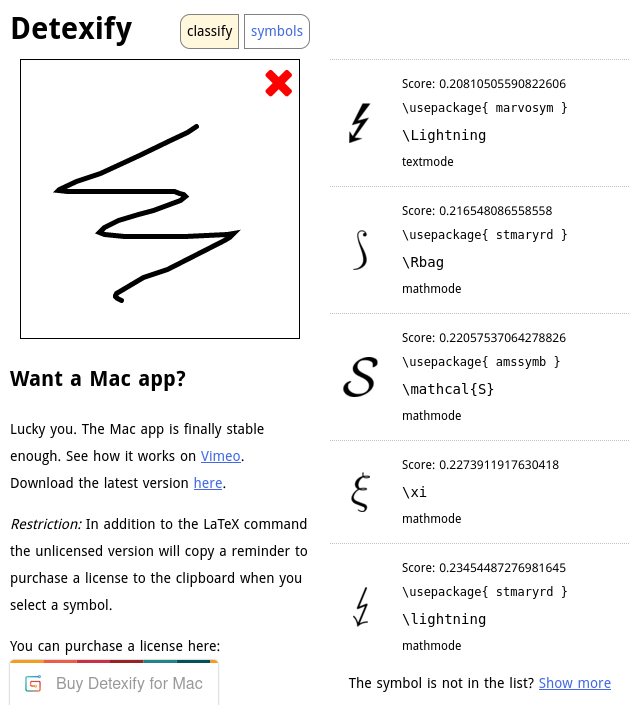
\includegraphics[scale=0.5]{./imagens/capitulo4/detexify.png}
		
	\end{center}
	\caption{Exemplo de uso da ferramenta \textit{online} detexify (\url{https://detexify.kirelabs.org/classify.html}).}
	\label{fig:detexify}
\end{figure}

Além dessas ferramentas, você pode utilizar o LyX\index{LyX} (\url{https://www.lyx.org/}), um editor de textos \gls{wysiwym}, que está disponível para Linux, Windows e Mac OS, e que é construído em cima do \LaTeX{}, e que permite se construir facilmente não só equações usando uma interface gráfica, mas também ambientes tabulares complexos para inserção em tabelas.

Finalmente, gostaria de indicar uma ferramenta simples, mas que pode ser bastante útil quando você quer incluir um símbolo matemático no seu documento mas esqueceu do nome dele em \LaTeX{}. Se este é o seu caso, visite a página do detexify\index{detexify}
\url{https://detexify.kirelabs.org/classify.html} e desenhe uma aproximação do símbolo no janela indicada e um software de classificação vai indicar quais símbolos são mais parecidos com o seu desenho, qual é o nome do comando que representa o símbolo e o pacote ao qual ele pertence. Um exemplo do uso desta ferramenta pode ser visto na Figura \ref{fig:detexify}.

\section{Provas} 

Existem vários pacotes que auxiliam na criação de provas de diversos estilos. Neste modelo, incorporamos alguns desses pacotes, os quais descrevemos brevemente a seguir. O primeiro pacote a ser apresentado é o \texttt{bussproofs}, um pacote que permite que se construa árvores de provas no estilo de cálculo de sequentes e outros sistemas de provas. Esse pacote define o comando \texttt{\textbackslash{}fCenter}, que define um ponto central para uso no alinhamento horizontal. Abaixo vemos um exemplo do uso do pacote \texttt{bussproofs}\index{bussproofs}, seguido dos comandos usados para gerá-lo, no Código \ref{cod:bussproofs}, inclusive do comando \texttt{\textbackslash{}fCenter}. 

\def\fCenter{\mbox{\Large$\rightarrow$}}
\begin{prooftree}
	\Axiom$\Gamma, A, B\ \fCenter\ B$
	\UnaryInf$\Gamma, A\ \fCenter\ (B \to C)$
	\UnaryInf$\Gamma\ \fCenter\ (A \to (B \to C))$
\end{prooftree}

\begin{listing}[ht]
	\begin{minted}[linenos=true, autogobble, bgcolor=Cornsilk1]{tex}
		\def\fCenter{\mbox{\Large$\rightarrow$}}
		\begin{prooftree}
		  \Axiom$\Gamma, A, B\ \fCenter\ B$
		  \UnaryInf$\Gamma, A\ \fCenter\ (B \to C)$
		  \UnaryInf$\Gamma\ \fCenter\ (A \to (B \to C))$
		\end{prooftree}
	\end{minted} 
	\caption{Exemplo do uso do pacote \texttt{bussproofs}. Exemplo extraído de \parencite{bussproofs}.}
	\label{cod:bussproofs}
\end{listing}

O endereço \url{http://mirrors.ctan.org/macros/latex/contrib/bussproofs/testbp2.pdf} permite que se acesse um pequeno documento contendo exemplos do uso do pacote enquanto que o manual pode ser acessado em \url{http://mirrors.ctan.org/macros/latex/contrib/bussproofs/BussGuide2.pdf} \parencite{bussproofs}.

Já o pacote \texttt{lplfitch}\index{lplfitch} provê macros para a diagramação de provas por dedução natural no estilo ``Fitch'', com as sub-provas indentadas e linhas de escopo. A tentativa do uso desse pacote com pacotes das classes de documentos do \gls{koma} gerou erros por conflito devido ao uso de pacotes descontinuados pelo \TeX{} mas que ainda funcionam com classes mais antigas como a \texttt{book}\index{book} e \texttt{article}\index{article}. Para que este pacote funcione com as classes do modelo \gls{koma}\index{\hologo{KOMAScript}}, as duas linhas do Código \ref{cod:lplfitch-setup} devem ser definidas no preâmbulo do seu documento.

\begin{listing}[ht]
	\begin{minted}[linenos=true, autogobble, bgcolor=Cornsilk1]{tex}
	\DeclareOldFontCommand{\sf}{\normalfont\sffamily}{\mathsf}
	\DeclareOldFontCommand{\bf}{\normalfont\bfseries}{\mathbf}
	\end{minted} 
	\caption{Comandos necessários para o uso do pacote \texttt{lplfitch} \parencite{lplfitch} com as classes do modelo \gls{koma}\index{\hologo{KOMAScript}}.}
	\label{cod:lplfitch-setup}
\end{listing}

O exemplo abaixo mostra uma prova no estilo produzido pelo pacote \texttt{lplfitch}\index{lplfitch}, que pode ser incluído em um objeto \texttt{float}\index{float} \texttt{figure}\index{figure} ou apresentado sozinho. Devido a como o pacote \texttt{lplfitch} foi implementado, sugiro que você coloque comandos escolhendo o espaçamento simples antes e duplo após a prova, como pode ser visto no Código \ref{cod:lplfitch}. Caso isso não seja feito, os espaços entre as linhas das provas ficam muito grandes e o efeito não é muito bom.

\singlespacing
\fitchprf{}{
	\subproof{\pline[1.]{\uni{x}{(Cube(x)\lif Small(x))}}}{
		\subproof{\pline[2.]{\exi{x}{Cube(x)}}}{
			\boxedsubproof[3.]{a}{Cube(a)}{
				\pline[4.]{Cube(a)\lif Small(a)}[\lalle{1}]\\
				\pline[5.]{Small(a)}[\life{4}{3}]\\
				\pline[6.]{\exi{x}{Small(x)}}[\lexii{5}]
			}
			\pline[7.]{\exi{x}{Small(x)}}[\lexie{2}{3--6}]
		}
		\pline[8.]{\exi{x}{Cube(x)}\lif \exi{x}{Small(x)}}[\lifi{2--7}]
	}
	\pline[9.]{\brokenform{(\uni{x}{(Cube(x)\lif Small(x))}\lif}{
			\formula{(\exi{x}{Cube(x)} \lif \exi{x}{Small(x)})}}}[\lifi{1--8}]
}
\doublespacing

\begin{listing}[ht]
	\begin{minted}[linenos=true, autogobble, bgcolor=Cornsilk1]{tex}
	\singlespacing
	\fitchprf{}{
	  \subproof{\pline[1.]{\uni{x}{(Cube(x)\lif Small(x))}}}{
	    \subproof{\pline[2.]{\exi{x}{Cube(x)}}}{
	      \boxedsubproof[3.]{a}{Cube(a)}{
	        \pline[4.]{Cube(a)\lif Small(a)}[\lalle{1}]\\
	        \pline[5.]{Small(a)}[\life{4}{3}]\\
	        \pline[6.]{\exi{x}{Small(x)}}[\lexii{5}]
	      }
	      \pline[7.]{\exi{x}{Small(x)}}[\lexie{2}{3--6}]
	    }
	    \pline[8.]{\exi{x}{Cube(x)}\lif \exi{x}{Small(x)}}[\lifi{2--7}]
	  }
	  \pline[9.]{\brokenform{(\uni{x}{(Cube(x)\lif Small(x))}\lif}{
	      \formula{(\exi{x}{Cube(x)} \lif \exi{x}{Small(x)})}}}[\lifi{1--8}]
	}
	\doublespacing
	\end{minted} 
	\caption{Comandos necessários para o uso do pacote \texttt{lplfitch} \parencite{lplfitch} com as classes do modelo \gls{koma}.}
	\label{cod:lplfitch}
\end{listing}

\bigskip

O manual do pacote \texttt{lplfitch}\index{lplfitch} pode ser acessado em \url{http://mirrors.ctan.org/macros/latex/contrib/lplfitch/lplfitch.pdf} \parencite{lplfitch}.

Diferente dos pacotes vistos acima, o pacote \texttt{natded}\index{natded} implementa ferramentas para criar provas de dedução natural nos estilos de Jaśkowski e Kalish-Montague. O exemplo exemplo abaixo mostra uma prova escrita no estilo de Kalish-Montague (exemplo extraído de \parencite{natded}) e os comandos usados para gerá-la podem ser vistos no Código \ref{cod:natded}. A Linha 2 do Código \ref{cod:natded} foi incluída para diminuir o espaçamento entre linhas pois o pacote \texttt{natded} gera caixas com linhas não contíguas quando o espaçamento é duplo, como neste modelo. 

\begin{equation*}
\setstretch{1.3}
\KMproof{
	\cbblk{
		\proofline{((( P \rightarrow Q ) \land (\neg R \rightarrow \neg Q ) ) \rightarrow ( P \rightarrow R ) ) }{2 -- 13
Conditionalization}
	}{
		\proofline{(( P \rightarrow Q ) \land (\neg R \rightarrow \neg Q ) )}{Supposition}
		\cbblk{
			\proofline{( P \rightarrow R ) }{4 -- 13 Conditionalization}
		}{
			\proofline{ P }{Supposition}
			\proofline{(( P \rightarrow Q ) \land (\neg R  \rightarrow \neg Q ) ) }{2 Repeat}
			\proofline{( P \rightarrow Q )}{5 Simplification}
			\proofline{ Q }{4, 6 Modus Ponens}
			\proofline{(\neg R \rightarrow \neg Q )}{5 Simplification}
			\cbblk{
				\proofline{ R }{10 -- 13 Reductio ad Absurdum}
			}{
				\proofline{\neg R }{ Supposition}
				\proofline{(\neg R \rightarrow \neg Q ) }{8 Repeat }
				\proofline{\neg Q }{10 , 11 Modus Ponens}
				\proofline{ Q }{7 Repeat}
			}
		}
	}
}
\end{equation*}



O pacote \texttt{natded}\index{natded} disponibiliza o manual em \url{http://mirrors.ctan.org/macros/latex/contrib/natded/natded.pdf} \parencite{natded}, de onde foi extraído o exemplo acima, e a documentação extra em \url{http://mirrors.ctan.org/macros/latex/contrib/natded/extended_doc.pdf} \parencite{natded-extra}.

\section{Especificações}

Especificações formais usam notações matemáticas para modelar precisamente as propriedades que um sistema computacional deve possuir. Existem várias linguagens criadas para descrever essa propriedades. Neste modelo, incorporamos os pacotes das linguagens CSP\index{CSP}, Z\index{Z} e Circus\index{Circus}. Caso você não necessite usá-las, comente os comandos \texttt{\textbackslash usepackage} correspondentes.
 
 \begin{listing}[ht]
 	\begin{minted}[linenos=true, autogobble, bgcolor=Cornsilk1]{tex}
\begin{equation*}
  \setstretch{1.3}
  \KMproof{
    \cbblk{
      \proofline{((( P \rightarrow Q ) \land (\neg R \rightarrow 
        \neg Q ) ) \rightarrow ( P \rightarrow R ) ) }{2 -- 13
        Conditionalization}
     }{
      \proofline{(( P \rightarrow Q ) \land (\neg R \rightarrow 
        \neg Q ) ) }{Supposition}
      \cbblk{
        \proofline{( P \rightarrow R ) }{4 -- 13 Conditionalization}
      }{
        \proofline{ P }{ Supposition }
        \proofline{(( P \rightarrow Q ) \land (\neg R  \rightarrow 
          \neg Q ) ) }{2 Repeat}
        \proofline{( P \rightarrow Q ) }{5 Simplification}
        \proofline{ Q }{4, 6 Modus Ponens }
        \proofline{(\neg R \rightarrow \neg Q ) }{5 Simplification}
        \cbblk{
          \proofline{ R }{10 -- 13 Reductio ad Absurdum }
        }{
          \proofline{\neg R }{ Supposition}
          \proofline{(\neg R \rightarrow \neg Q ) }{8 Repeat}
          \proofline{\neg Q }{10 , 11 Modus Ponens}
          \proofline{ Q }{7 Repeat}
        }
      }
    }
 }
\end{equation*}
 	\end{minted} 
 	\caption{Exemplo do uso do pacote \texttt{natded}.}
 	\label{cod:natded}
 \end{listing}

O pacote \texttt{zed-csp}\index{zed-csp} é um pacote que foi desenvolvido baseado no pacote original \texttt{zed}\index{zed}, que implementa a diagramação no formato da linguagem Z\index{Z} e incluiu as definições para CSP\index{CSP}. O exemplo abaixo mostra o uso do ambiente de definição genérica (\texttt{gendef}\index{gendef}), criado pelo pacote \texttt{zed-csp}\index{zed-csp}, e os comandos usados para gerar este exemplo, extraído de \parencite{zed}\index{zed}, podem ser vistos no Código \ref{cod:zed-csp}.
 
\begin{gendef}[X,Y]
	first: X \cross Y \fun X
\where
		\forall x: X; y: Y @ \\
\t1     first(x,y) = x
\end{gendef}

\begin{listing}[ht]
	\begin{minted}[linenos=true, autogobble, bgcolor=Cornsilk1]{tex}
		\begin{gendef}[X,Y]
		  first: X \cross Y \fun X
		\where
		  \forall x: X; y: Y @ \\
		\t1     first(x,y) = x
		\end{gendef}
	\end{minted} 
	\caption{Exemplo do uso do pacote \texttt{zed-csp}.}
	\label{cod:zed-csp}
\end{listing}

O pacote \texttt{zed-csp}\index{zed-csp} possui dois manuais, um para a linguagem CSP\index{CSP} \url{http://mirrors.ctan.org/macros/latex/contrib/zed-csp/csp2e.pdf} \parencite{csp} e o outro para Z\index{Z} \url{http://mirrors.ctan.org/macros/latex/contrib/zed-csp/zed2e.pdf} \parencite{zed}. 

Existe um outro pacote para a criação de especificações em Z\index{Z}, o \texttt{objectz}\index{objectz}. Entretanto eu não carreguei ambos os pacotes para verificar se \texttt{objectz} e \texttt{zed-csp} são compatíveis, já que definem ambientes com os mesmos nomes. Caso precise usar o \texttt{objectz}, eu sugiro que apenas substitua o pacote \texttt{zed-csp}\index{zed-csp}. O manual do \texttt{objectz} pode ser acessado em \url{http://mirrors.ctan.org/macros/latex/contrib/objectz/ozguide.pdf} \parencite{objectz}.





